\documentclass[12pt,a4paper]{article}
\usepackage{geometry}
\usepackage[numbers]{natbib}
\usepackage{amssymb, amsmath}
\usepackage{graphicx}
\usepackage{grffile}
\graphicspath{{../Figures/}}
\usepackage{gensymb}
\usepackage[font=small]{caption}
\usepackage[utf8]{inputenc}
\usepackage[english]{babel}
\usepackage{fancyhdr}
\usepackage[raggedright]{titlesec}
\usepackage{subcaption}
\usepackage{multirow}
\usepackage{dirtytalk}
\usepackage{framed}
\usepackage[normalem]{ulem}
\usepackage[pdftex,breaklinks]{hyperref}
\hypersetup{
  colorlinks   = true, %Colours links instead of ugly boxes
  urlcolor     = green, %Colour for external hyperlinks
  linkcolor    = blue, %Colour of internal links
  citecolor   = red %Colour of citations
}


\begin{document}
\author{Katrina Ashton}


\pagestyle{fancy}
\fancyhf{}
\rhead{\thepage}
\lhead{u5586882}

\section{What I've done}
\begin{itemize}
  \item Worked on my report.
  \item Captured new trajectory (square with sides 1m) with new scene (different small box, carpet on ground)
  \item Captured another circle trajectory with new scene (same as square trajectory)
  \item Initial results for new trajectories (need to play around with some of the frequency stuff to get it to work)
  \item Started planning out seminar slides
\end{itemize}

\section{Parts of report to look at}
\begin{itemize}
\item Intro, lit review, background info
\end{itemize}

\section{Questions}
\begin{itemize}
\item Should I see what performance is like with different features? (I'm currently using SIFT)
\item Should I add a section in the background info about features?
\item Is it worth trying to get ICP working or should I just cut it? Could also try use it to refine an estimate from one of the other methods rather than by itself (which is how it seems to be used in practice). Although not sure I'll have time to actually implement that.
\end{itemize}

\section{Comments}
\begin{itemize}
  \item Need to try some stuff to see if I can get better trajectories (see Figure \ref{f: quad square trj})
  \item Essential Matrix seems to be going ok until it hits the last side and gets turned around.
  \item PnP seems to be doing some kind of weird cross-over thing and the side are too big.
  \item Kabsch is complete nonsense (but can't see boxes during the turns and some of the straight sections, so somewhat expected?)
\end{itemize}



     \begin{figure}[p]
      \begin{subfigure}[t]{0.5\textwidth}
      \centering
        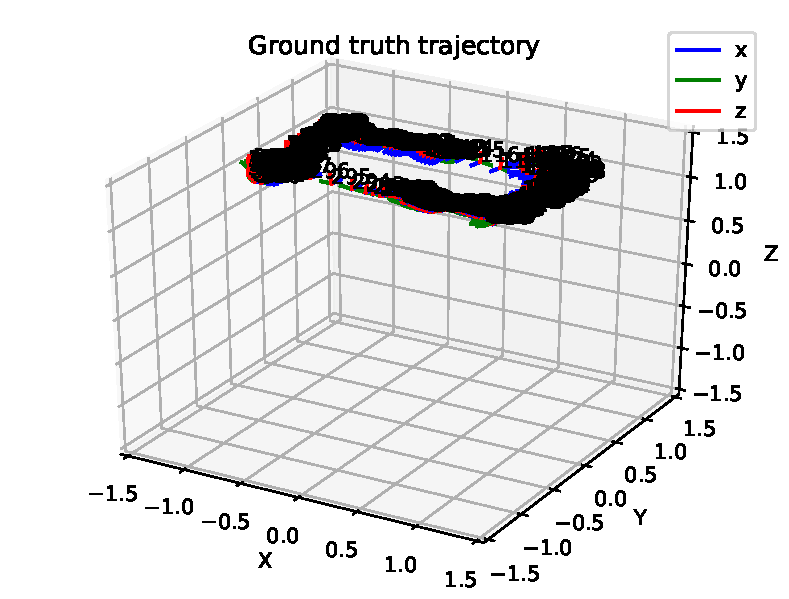
\includegraphics[width=80mm]{../quad/basic-reg-saves-S1b/5/atrj_gt.pdf}
        \caption{Ground truth trajectory (skip 5)}
      \end{subfigure} %
      ~
      \begin{subfigure}[t]{0.5\textwidth}
        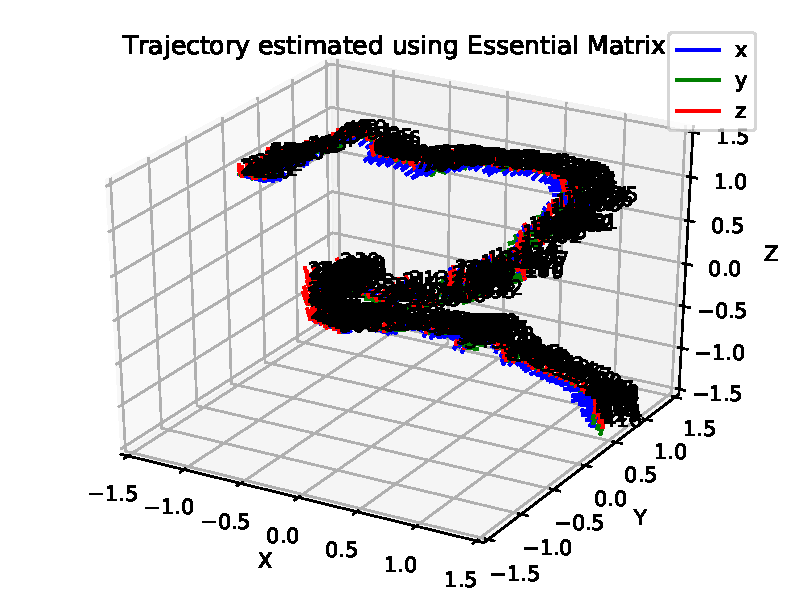
\includegraphics[width=80mm]{../quad/basic-reg-saves-S1b/5/atrj_rgb.pdf}
        \caption{Trajectory estimated by Essential Matrix method}
      \end{subfigure} 
      \\
      \begin{subfigure}[t]{0.5\textwidth}
        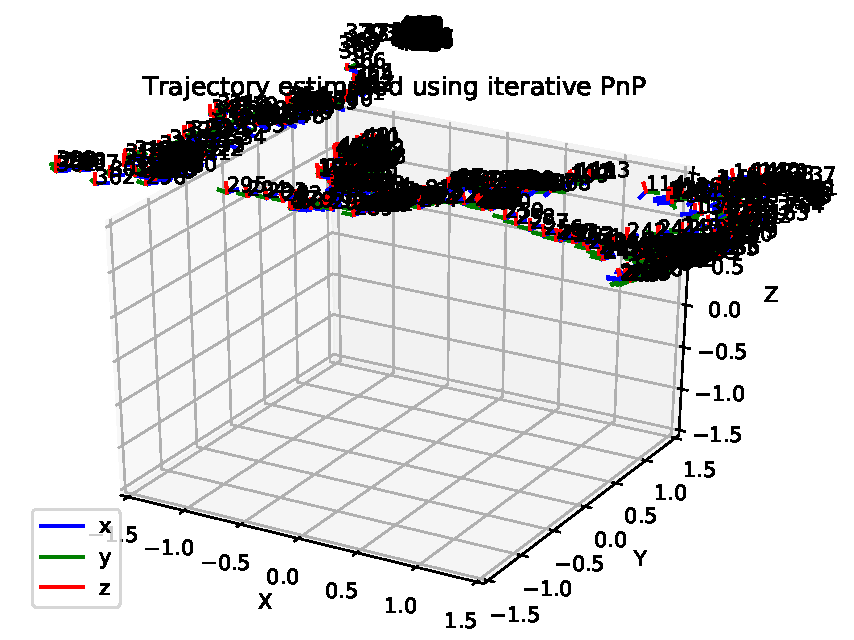
\includegraphics[width=80mm]{../quad/basic-reg-saves-S1b/5/atrj_pnp.pdf}
        \caption{Trajectory estimated by PnP}
      \end{subfigure} %
      ~
      \begin{subfigure}[t]{0.5\textwidth}
        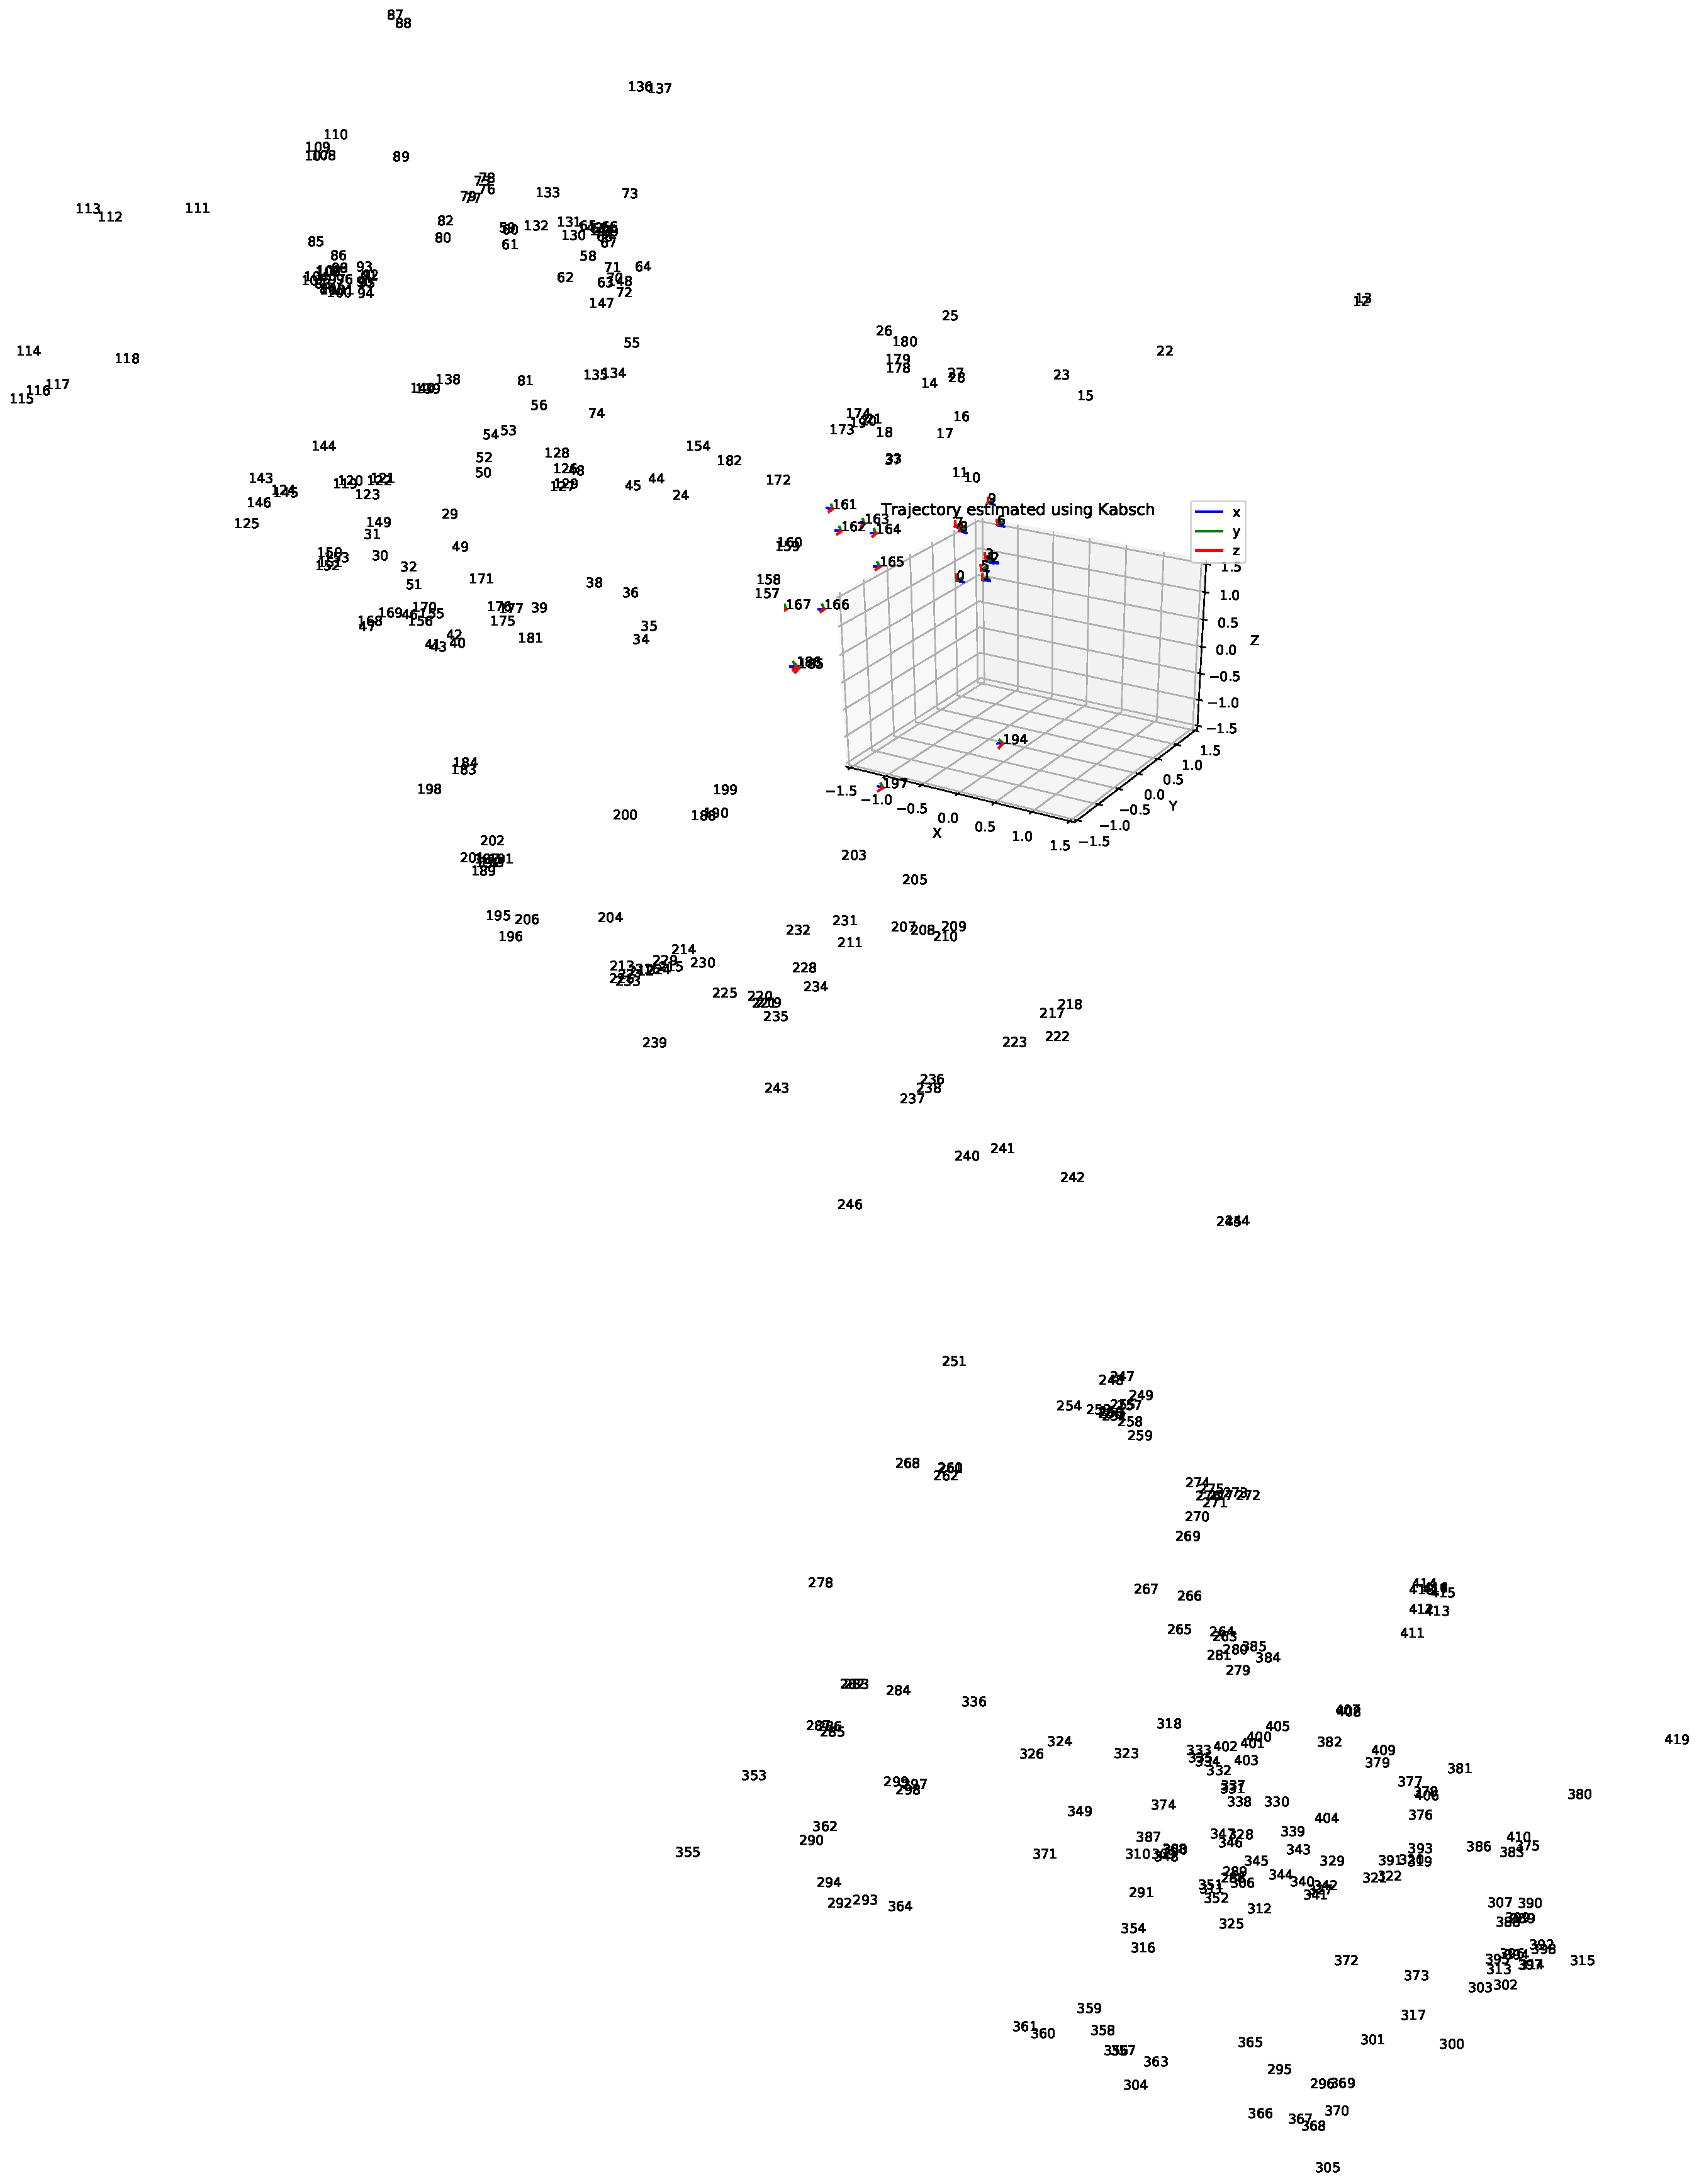
\includegraphics[width=80mm]{../quad/basic-reg-saves-S1b/5/atrj_d.pdf}
        \caption{Trajectory estimated by Kabsch}
      \end{subfigure}
      \caption{Trajectories for square trajectory (1m sides), with 5 frames skipped only one loop.}
      \label{f: quad square trj}
    \end{figure}


\bibliographystyle{abbrvnat}
\bibliography{../Report/ENGN4217}

\end{document}